% Research Diary Collection Template for Research Student (University), 2025
\documentclass[letterpaper,11pt]{article}
\newcommand{\userName}{Research Student}
\newcommand{\institution}{University}
\newcommand{\workingDate}{2025 Research Diary}
% Modular package loading - choose what you need
% Files are symlinked in output directory for self-contained compilation

\usepackage{assets/styles/diary_base}        % Core packages and basic theorems
\usepackage{assets/styles/diary_ctheorems}   % Enhanced colored theorem environments
\usepackage{assets/styles/diary_commands}   % Personal shortcuts and commands

\usepackage{tocloft}
\setlength{\cftbeforesecskip}{5pt}
\renewcommand*\contentsname{Research Student's Research Diary -- Contents}

\title{Research Diary Collection - 2025}
\author{Research Student}
\date{Compiled \today}

\begin{document}

\tableofcontents
\thispagestyle{empty}
\newpage


% Entry from 2025-09-20-newmethod.tex
\href{run:2025-09-20-newmethod.tex}{\Huge September 20} 

\section{Machine Learning}

We have a citation \cite{research_methods2024} here.  Solve this problem: 

\bb 
\min_{\theta} \sum_{i=1}^n (f_\theta(x\datai) - y\datai)^2. 
\ee 


\clearpage


% Entry from 2025-09-20.tex
\href{run:2025-09-20.tex}{\Huge September 20} 

\section{Rectified Flow}

We have a figure here. 
\begin{figure}[h]
\centering 
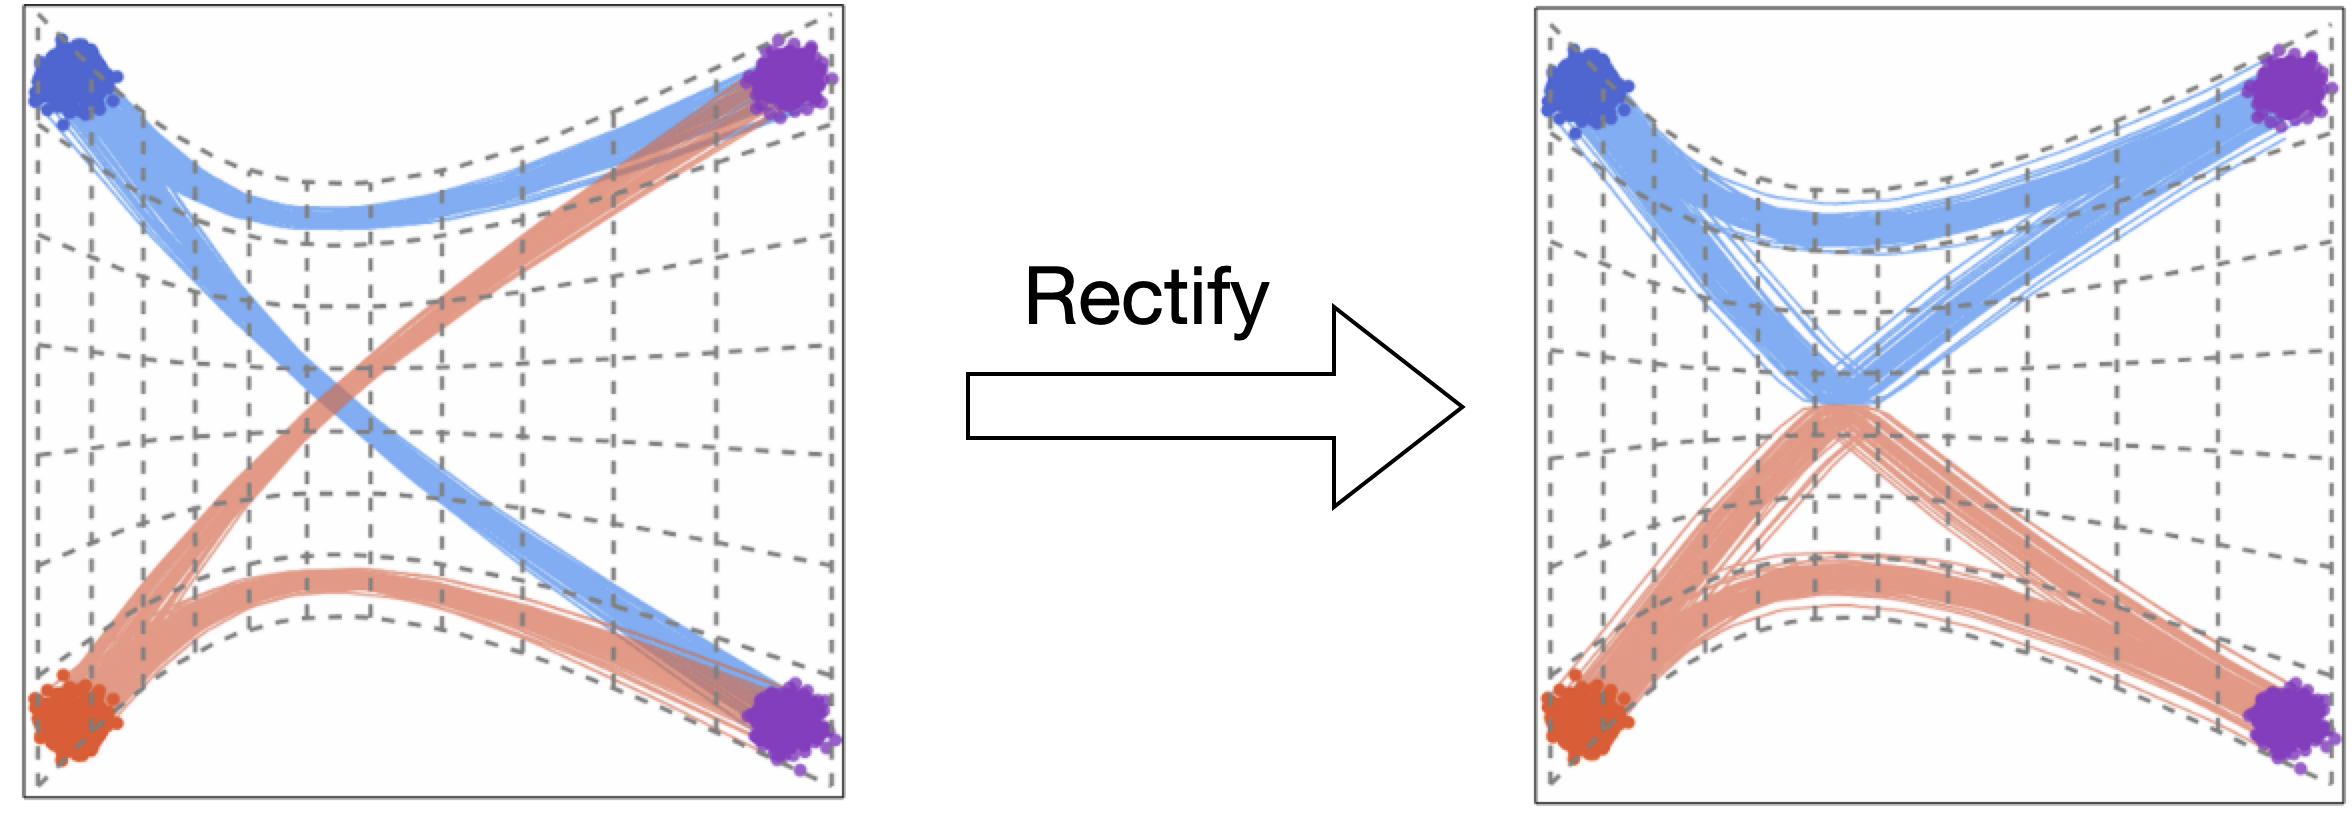
\includegraphics[width=0.8\textwidth]{assets/figures/2025/curved_reflow.png}
\end{figure} 


We have another citation here \cite{li2022diffusion}. 


\clearpage


% Entry from 2025-09-21.tex
\href{run:2025-09-21.tex}{\Huge September 21} 

\section{Today is a New Day}

Dealing with math, code, people, self. 



\clearpage


\bibliographystyle{apalike}
\bibliography{assets/bib/reference,assets/bib/reference2}


\end{document}
